% Template for PLoS
% Version 3.5 March 2018
%
% % % % % % % % % % % % % % % % % % % % % %
%
% -- IMPORTANT NOTE
%
% This template contains comments intended
% to minimize problems and delays during our production
% process. Please follow the template instructions
% whenever possible.
%
% % % % % % % % % % % % % % % % % % % % % % %
%
% Once your paper is accepted for publication,
% PLEASE REMOVE ALL TRACKED CHANGES in this file
% and leave only the final text of your manuscript.
% PLOS recommends the use of latexdiff to track changes during review, as this will help to maintain a clean tex file.
% Visit https://www.ctan.org/pkg/latexdiff?lang=en for info or contact us at latex@plos.org.
%
%
% There are no restrictions on package use within the LaTeX files except that
% no packages listed in the template may be deleted.
%
% Please do not include colors or graphics in the text.
%
% The manuscript LaTeX source should be contained within a single file (do not use \input, \externaldocument, or similar commands).
%
% % % % % % % % % % % % % % % % % % % % % % %
%
% -- FIGURES AND TABLES
%
% Please include tables/figure captions directly after the paragraph where they are first cited in the text.
%
% DO NOT INCLUDE GRAPHICS IN YOUR MANUSCRIPT
% - Figures should be uploaded separately from your manuscript file.
% - Figures generated using LaTeX should be extracted and removed from the PDF before submission.
% - Figures containing multiple panels/subfigures must be combined into one image file before submission.
% For figure citations, please use "Fig" instead of "Figure".
% See http://journals.plos.org/plosone/s/figures for PLOS figure guidelines.
%
% Tables should be cell-based and may not contain:
% - spacing/line breaks within cells to alter layout or alignment
% - do not nest tabular environments (no tabular environments within tabular environments)
% - no graphics or colored text (cell background color/shading OK)
% See http://journals.plos.org/plosone/s/tables for table guidelines.
%
% For tables that exceed the width of the text column, use the adjustwidth environment as illustrated in the example table in text below.
%
% % % % % % % % % % % % % % % % % % % % % % % %
%
% -- EQUATIONS, MATH SYMBOLS, SUBSCRIPTS, AND SUPERSCRIPTS
%
% IMPORTANT
% Below are a few tips to help format your equations and other special characters according to our specifications. For more tips to help reduce the possibility of formatting errors during conversion, please see our LaTeX guidelines at http://journals.plos.org/plosone/s/latex
%
% For inline equations, please be sure to include all portions of an equation in the math environment.
%
% Do not include text that is not math in the math environment.
%
% Please add line breaks to long display equations when possible in order to fit size of the column.
%
% For inline equations, please do not include punctuation (commas, etc) within the math environment unless this is part of the equation.
%
% When adding superscript or subscripts outside of brackets/braces, please group using {}.
%
% Do not use \cal for caligraphic font.  Instead, use \mathcal{}
%
% % % % % % % % % % % % % % % % % % % % % % % %
%
% Please contact latex@plos.org with any questions.
%
% % % % % % % % % % % % % % % % % % % % % % % %

\documentclass[10pt,letterpaper]{article}
\usepackage[top=0.85in,left=2.75in,footskip=0.75in]{geometry}

% amsmath and amssymb packages, useful for mathematical formulas and symbols
\usepackage{amsmath,amssymb}

% Use adjustwidth environment to exceed column width (see example table in text)
\usepackage{changepage}

% Use Unicode characters when possible
\usepackage[utf8x]{inputenc}

% textcomp package and marvosym package for additional characters
\usepackage{textcomp,marvosym}

% cite package, to clean up citations in the main text. Do not remove.
% \usepackage{cite}

% Use nameref to cite supporting information files (see Supporting Information section for more info)
\usepackage{nameref,hyperref}

% line numbers
\usepackage[right]{lineno}

% ligatures disabled
\usepackage{microtype}
\DisableLigatures[f]{encoding = *, family = * }

% color can be used to apply background shading to table cells only
\usepackage[table]{xcolor}

% array package and thick rules for tables
\usepackage{array}

% create "+" rule type for thick vertical lines
\newcolumntype{+}{!{\vrule width 2pt}}

% create \thickcline for thick horizontal lines of variable length
\newlength\savedwidth
\newcommand\thickcline[1]{%
  \noalign{\global\savedwidth\arrayrulewidth\global\arrayrulewidth 2pt}%
  \cline{#1}%
  \noalign{\vskip\arrayrulewidth}%
  \noalign{\global\arrayrulewidth\savedwidth}%
}

% \thickhline command for thick horizontal lines that span the table
\newcommand\thickhline{\noalign{\global\savedwidth\arrayrulewidth\global\arrayrulewidth 2pt}%
\hline
\noalign{\global\arrayrulewidth\savedwidth}}


% Remove comment for double spacing
%\usepackage{setspace}
%\doublespacing

% Text layout
\raggedright
\setlength{\parindent}{0.5cm}
\textwidth 5.25in
\textheight 8.75in

% Bold the 'Figure #' in the caption and separate it from the title/caption with a period
% Captions will be left justified
\usepackage[aboveskip=1pt,labelfont=bf,labelsep=period,justification=raggedright,singlelinecheck=off]{caption}
\renewcommand{\figurename}{Fig}

% Use the PLoS provided BiBTeX style
% \bibliographystyle{plos2015}

% Remove brackets from numbering in List of References
\makeatletter
\renewcommand{\@biblabel}[1]{\quad#1.}
\makeatother



% Header and Footer with logo
\usepackage{lastpage,fancyhdr,graphicx}
\usepackage{epstopdf}
%\pagestyle{myheadings}
\pagestyle{fancy}
\fancyhf{}
%\setlength{\headheight}{27.023pt}
%\lhead{
\includegraphics[width=2.0in]{PLOS-submission.eps}}
\rfoot{\thepage/\pageref{LastPage}}
\renewcommand{\headrulewidth}{0pt}
\renewcommand{\footrule}{\hrule height 2pt \vspace{2mm}}
\fancyheadoffset[L]{2.25in}
\fancyfootoffset[L]{2.25in}
\lfoot{\today}

%% Include all macros below

\newcommand{\lorem}{{\bf LOREM}}
\newcommand{\ipsum}{{\bf IPSUM}}


% Pandoc citation processing
\newlength{\csllabelwidth}
\setlength{\csllabelwidth}{3em}
\newlength{\cslhangindent}
\setlength{\cslhangindent}{1.5em}
% for Pandoc 2.8 to 2.10.1
\newenvironment{cslreferences}%
  {}%
  {\par}
% For Pandoc 2.11+
\newenvironment{CSLReferences}[3] % #1 hanging-ident, #2 entry spacing
 {% don't indent paragraphs
  \setlength{\parindent}{0pt}
  % turn on hanging indent if param 1 is 1
  \ifodd #1 \everypar{\setlength{\hangindent}{\cslhangindent}}\ignorespaces\fi
  % set entry spacing
  \ifnum #2 > 0
  \setlength{\parskip}{#2\baselineskip}
  \fi
 }%
 {}
\usepackage{calc} % for calculating minipage widths
\newcommand{\CSLBlock}[1]{#1\hfill\break}
\newcommand{\CSLLeftMargin}[1]{\parbox[t]{\csllabelwidth}{#1}}
\newcommand{\CSLRightInline}[1]{\parbox[t]{\linewidth - \csllabelwidth}{#1}}
\newcommand{\CSLIndent}[1]{\hspace{\cslhangindent}#1}

\usepackage{booktabs}
\usepackage{longtable}
\usepackage{array}
\usepackage{multirow}
\usepackage{wrapfig}
\usepackage{float}
\usepackage{colortbl}
\usepackage{pdflscape}
\usepackage{tabu}
\usepackage{threeparttable}
\usepackage{threeparttablex}
\usepackage[normalem]{ulem}
\usepackage{makecell}
\usepackage{xcolor}



\usepackage{forarray}
\usepackage{xstring}
\newcommand{\getIndex}[2]{
  \ForEach{,}{\IfEq{#1}{\thislevelitem}{\number\thislevelcount\ExitForEach}{}}{#2}
}

\setcounter{secnumdepth}{0}

\newcommand{\getAff}[1]{
  \getIndex{#1}{McMaster University}
}

\providecommand{\tightlist}{%
  \setlength{\itemsep}{0pt}\setlength{\parskip}{0pt}}

\begin{document}
\vspace*{0.2in}

% Title must be 250 characters or less.
\begin{flushleft}
{\Large
\textbf\newline{The importance of reproducibility in COVID-19 research:
the case of population density and the spread of the
pandemic} % Please use "sentence case" for title and headings (capitalize only the first word in a title (or heading), the first word in a subtitle (or subheading), and any proper nouns).
}
\newline
% Insert author names, affiliations and corresponding author email (do not include titles, positions, or degrees).
\\
Antonio Paez\textsuperscript{\getAff{McMaster
University}}\textsuperscript{*}\\
\bigskip
\textbf{\getAff{McMaster University}}School of Earth, Environment and
Society, 1280 Main St West, Hamilton, Ontario L8S 4K1 Canada\\
\bigskip
* Corresponding author: paezha@mcmaster.ca\\
\end{flushleft}
% Please keep the abstract below 300 words
\section*{Abstract}
The emergence of the novel SARS-CoV-2 coronavirus and the global
COVID-19 pandemic has led to explosive growth in scientific research.
Given the high stakes of the situation, it is essential that scientific
activites, on which good policy depends, are as transparent and
reproducible as possible. Reproducibility is key for the efficient
operation of the self-correction mechanisms of science, which work to
weed out errors and refine our understanding of social and physical
phenomena. In this paper, the importance of reproducibility is
illustrated for the case of the association between population density
and the the spread of SARS-CoV-2. Transparency and openness means that
the same problem can, with relatively modest efforts, be examined by
independent researchers who can verify findings, and bring to bear
different perspectives, approaches, and methods---sometimes with
consequantial changes in the conclusions, as the empirical example in
this paper shows.

% Please keep the Author Summary between 150 and 200 words
% Use first person. PLOS ONE authors please skip this step.
% Author Summary not valid for PLOS ONE submissions.

\linenumbers

% Use "Eq" instead of "Equation" for equation citations.
\hypertarget{introduction}{%
\section{Introduction}\label{introduction}}

The emergence of the novel SARS-CoV-2 coronavirus in 2019, and the
global pandemic that followed in its wake, led to an explosive growth of
research. According to Fraser et al. {[}1{]}, over 125,000
COVID-19-related papers were released in the first ten months from the
first confirmed case of the disease. Of these, more than 30,000 were
shared in pre-print servers, the use of which also exploded in the past
year {[}2--4{]}.

Given the heavy human and economic cost of the pandemic, there has been
a natural tension in the scientific community between the need to
publish research results quickly and the imperative to maintain
consistently high quality standards in scientific reporting; indeed, a
call for maintaining the standards in published research has even called
this deluge of publications a ``carnage of substandard research''
{[}5{]}. Part of the challenge of maintaining quality standards in
published research is that, despite an abundance of recommendations and
guidelines {[}6--9{]}, in practice reproducibility has remained a lofty
and somewhat aspirational goal {[}10,11{]}. As reported in the
literature, only a woefully small proportion of published research was
actually reproducible before the pandemic {[}12,13{]}, and the situation
does not appear to have changed substantially since {[}14,15{]}.

The push for open data and software, along with more strenuous efforts
towards open, reproducible research, is simply a continuation of
long-standing scientific practices of independent verification. Despite
the (at times disproportionate) attention that high profile scandals in
science tend to elicit in the media, science as a collective endeavor is
remarkable for being a self-correcting enterprise, one with built-in
mechanisms and incentives to weed out erroneous ideas. Over the long
term, facts tend to prevail in science. At stake is the shorter-term
impacts that research may have in other spheres of economic and social
life. The case of economists Reinhart and Rogoff comes to mind: by the
time the inaccuracies and errors in their research were uncovered {[}see
16{]}, their claims about debt and economic growth had already been
seized by policy-makers on both sides of the Atlantic to justify
austerity policies in the aftermath of the Great Recession of
2007-2009\footnote{Nobel Prize in Economics Paul Krugman noted that
  ``Reinhart--Rogoff may have had more immediate influence on public
  debate than any previous paper in the history of economics''
  \url{https://www.nybooks.com/articles/2013/06/06/how-case-austerity-has-crumbled/?pagination=false}}.
As later research has demonstrated, those policies cast a long shadow,
and their sequels continued to be felt for years {[}17{]}.

In the context of COVID-19, a topic that has grabbed the imagination of
numerous thinkers has been the prospect of life in cities after the
pandemic {[}18{]}. The fact that the worst of the pandemic was initially
felt in dense population centers such as Wuhan, Milan, Madrid, and New
York, brought a torrent of research into the associations between
density and the spread of the pandemic. Some important questions hang on
the results of these research efforts. For example, are lower density
regions safer from the pandemic? Are de-densification policies
warranted, at least in the short term? And in the longer term, will the
risks of life in high density regions presage a flight from cities? Over
the past year, numerous papers have sought to throw light into the
underlying issue of density and the pandemic; nonetheless the results,
as will be detailed next, remain mixed. Further, to complicate matters,
precious few of these studies appear to be sufficiently open to support
independent verification.

The objective of this paper is to illustrate the importance of
reproducibility in research, particularly in the context of the flood of
COVID-19 papers. To this end, a recent study by Sy et al. {[}19{]} is
chosen as an example of reproducible research. The objective is not to
malign the analysis of these researchers, but rather to demonstrate the
value of openness to allow for independent verification and further
analysis. Open data and open code mean that an independent researcher
can, with only modest efforts, not only verify the findings reported,
but also examine the same data from a perspective which may not have
been available to the original researchers due to differences in
disciplinary perspectives, methodological traditions, and/or training,
among other possible factors. The example, which shows consequential
changes in the conclusions reached by different analyses, should serve
as a call to researchers to redouble their efforts to increase
transparency and reproducibility in research. This paper, in addition,
aims to show how data can be packaged in well-documented, shareable
units, and code can be embedded into self-contained documents suitable
for review and independent verification. The source for this paper is an
\href{http://rmarkdown.rstudio.com}{R Markdown} document which, along
with the data package, is available in a public repository\footnote{\url{https://github.com/paezha/Reproductive-Rate-and-Density-US-Reanalyzed}}.

\hypertarget{background}{%
\section{Background}\label{background}}

The concern with population density and the spread of the virus during
the COVID-19 pandemic was fueled, at least in part, by dramatic scenes
seen in real-time around the world from large urban centers such as
Wuhan, Milan, Madrid, and New York. In theory, there are good reasons to
believe that higher density may have a positive association with the
transmission of a contagious virus. It has long been known that the
potential for inter-personal contact is greater in regions with higher
density {[}see for example the research on urban fields and
time-geography 20,21,22{]}. Mathematically, models of exposure and
contagion indicate that higher densities can catalyze the transmission
of contagious diseases {[}23,24{]}. Models such as these were likely at
the root of messages, by some figures in positions of authority, that
regions with sparse population densities faced lower risks from the
pandemic\footnote{Governor Kristi Noem of South Dakota, for example,
  claimed that sparse population density allowed her state to face the
  pandemic down without the need for strict policy interventions
  \url{https://www.inforum.com/lifestyle/health/5025620-South-Dakota-is-not-New-York-City-Noem-defends-lack-of-statewide-COVID-19-restrictions}}.

As Rocklöv and Sjödin {[}23{]} note, however, mathematical models of
contagion are valid at small-to-medium spatial scales (and presumably,
small temporal scales too, such as time spent in restaurants, concert
halls, cruises), and the results do not necessarily transfer to larger
spatial units and different time scales. There are solid reasons for
this: while in a restaurant, one can hardly avoid being in proximity to
other customers-however, a person can choose to (or be forced to as a
matter of policy) not go to a restaurant in the first place.
Nonetheless, the idea that high density correlates with high
transmission is so intuitive that it is often taken for granted even at
larger scales {[}e.g., 25,26{]}. At larger scales, however, there exists
the possibility of behavioral adaptations, which are difficult to
capture in the mechanistic framework of differential equations {[}or can
be missing in agent-based models, e.g., 27{]}; these adaptations, in
fact, can be a key aspect of disease transmission.

A plausible behavioral adaptation during a pandemic, especially one
broadcast as widely and intensely as COVID-19, is risk compensation.
Risk compensation is a process whereby people adjust their behavior in
response to their \emph{perception} of risk {[}28--30{]}. In the case of
COVID-19, Chauhan et al. {[}31{]} have found that perception of risks in
the US varies between rural, suburban, and urban residents, with rural
residents in general expressing less concern about the virus. It is
possible that people who listened to the message of leaders saying that
they were safe because of low density may not have taken adequate
precautions against the virus. People in dense places who could more
directly observe the impact of the pandemic may have become overly
cautious. Both Paez et al. {[}32{]} and Hamidi et al. {[}33{]} posit
this mechanism (i.e., greater compliance with social distancing in
denser regions) to explain the results of their analyses. The evidence
available does indeed show that there were important changes in behavior
with respect to mobility during the pandemic {[}34--36{]}; furthermore,
shelter in place orders may have had greater buy-in from the public in
higher density regions {[}37{]}, and the associated behavior may have
persisted beyond the duration of official social-distancing policies
{[}38{]}. In addition, there is evidence that changes in mobility
correlated with the trajectory of the pandemic {[}39,40{]}. Given the
potential for behavioral adaptation, the question of density becomes
more nuanced: it is not just a matter of proximity, but also of human
behavior, which is better studied using population-level data and
models.

In this respect, the literature to date remains inconclusive.

On the one hand, there are studies that report positive associations
between population density and various COVID-19-related outcomes. Bhadra
{[}41{]}, for example, reported a moderate positive correlation between
the spread of COVID-19 and population density at the district level in
India, however their analysis was bivariate and did not control for
other variables, such as income. Similarly, Kadi and Khelfaoui {[}42{]}
found a positive and significant correlation between number of cases and
population density in cities in Algeria in a series of simple regression
models (i.e., without other controls). A question in these relatively
simple analyses is whether density is not a proxy for other factors.
Other studies have included controls, such as Pequeno et al. {[}43{]}, a
team that reported a positive association between density and cumulative
counts of confirmed COVID-19 cases in state capitals in Brazil after
controlling for covariates, including income, transport connectivity,
and economic status. In a similar vein, Fielding-Miller et al. {[}44{]}
reported a positive relationship between the absolute number of COVID-19
deaths and population density (rate) in rural counties in the US. Roy
and Ghosh {[}45{]} used a battery of machine learning techniques to find
discriminatory factors, and a positive and significant association
between COVID-19 infection and death rates in US states. Wong and Li
{[}46{]} also found a positive and significant association between
population density and number of confirmed COVID-19 cases in US
counties, using both univariate and multivariate regressions with
spatial effects. More recently, Sy et al. {[}19{]} reported that the
basic reproductive number of COVID-19 in US counties tended to increase
with population density, but at a decreasing rate at higher densities.

On the flip side, a number of studies report non-significant or negative
associations between population density and COVID-19 outcomes. This
includes the research of Sun et al. {[}47{]} who did not find evidence
of significant correlation between population density and confirmed
number of cases per day \emph{in conditions of lockdown} in China. This
finding echoes the results of Paez et al. {[}32{]}, who in their study
of provinces in Spain reported non-significant associations between
population density and infection rates in the early days of the first
wave of COVID-19, and negative significant associations in the later
part of the first lockdown. Similarly, {[}48{]} found zero or negative
associations between population density and infection numbers/deaths by
country. Fielding-Miller et al. {[}44{]} contrast their finding about
rural counties with a negative relationship between COVID-19 deaths and
population density in urban counties in the US. For their part, in their
investigation of doubling time, White and Hébert-Dufresne {[}49{]}
identified a negative and significant correlation between population
density and doubling time in US states. Likewise, {[}50{]} fond a small
negative (and significant) association between population density and
COVID-19 morbidity in districts in Tehran. Finally, two of the most
complete studies in the US {[}by Hamidi et al.; {[}51{]}; {[}33{]}{]}
used an extensive set of controls to find negative and significant
correlations between density and COVID-19 cases and fatalities at the
level of counties in the US.

As can be seen, these studies are implemented at different scales in
different regions of the world. They also use a range of techniques,
from correlation analysis, to multivariate regression, spatial
regressions, and machine learning techniques. This is natural and to be
expected: individual researchers have only limited time and expertise.
This is why reproducibility is important. To pick an example (which will
be further elaborated in the following sections), the study of Sy et
al.~{[}{[}19{]}; hereafter SWN{]} would immediately grab the attention
of a researcher with expertise in spatial modelling.

SWN investigated the basic reproductive number of COVID-19 in US
counties, and its association with population density, median household
income, and prevalence of private mobility. The basic reproductive
number can only be calculated reliably with a minimum number of cases,
and a large number of counties did not meet such threshold. As
researchers do, SWN made certain seemingly reasonable modelling
decision, for instance basing their analysis only on counties with valid
observations. An experiences spatial modeler would likely ask some of
the following questions on reading SWN's paper: how were missing
counties treated? Is it possible to spatially interpolate the missing
observations? What are the implications of the spatial sampling
framework used in the analysis? And, was there evidence of spatial
autocorrelation in the residuals of the models? These are questions that
in most cases would not occur to a researcher who has not been exposed
to spatial statistics or spatial econometrics. Nonetheless, they are
relevant and important. Fortunately, SWN give an example of a reasonably
open, reproducible research product: their paper is accompanied by (most
of) the data and (most of) the code used in the analysis. This means
that an independent expert can, with only a moderate investment of time
and effort, replicate the results in the paper, as well as ask
additional questions.

Alas, reproducibility is not necessarily the norm in the relevant
literature.

There are various reasons why a project can fail to be reproducible. In
some cases, there might be legitimate reasons to withhold the data,
perhaps due to confidentiality and privacy reasons {[}e.g., 52{]}. But
in many other cases the data are publicly available, which in fact has
commonly been the case with population-level COVID-19 information.
Typically the provenance of the data is documented, but in numerous
studies the data themselves are not shared {[}25,33,41,44,51,53--56{]}.
As any researcher can attest, whether a graduate student or a seasoned
scientist, collecting, organizing, and preparing data for a project can
take a substantial amount of time. Pointing to the sources of data, even
when these sources are public, is a small step towards
reproducibility-but only a very small one. Faced with the prospect of
having to recreate a data set from raw sources is probably sufficient to
dissuade all but the most dedicated (or stubborn) researcher from
independent verification. This is true even if part of the data are
shared {[}e.g., 46{]}. In other cases, data are shared, but the
processes followed in the preparation of the data are not fully
documented {[}48,57{]}. These processes matter, as shown by the errors
in the spreadsheets of Reinhart and Rogoff {[}16{]} and the data of
biologist Jonathan Pruitt that led to an ``avalanche'' of paper
retractions\footnote{\url{https://doi.org/10.1038/d41586-020-00287-y}}.
Another situation is when papers share well-documented data, but fail to
provide the code used in the analysis {[}43,58,59{]}. Making code
available only ``on demand'' {[}e.g., 60{]} is an unnecessary barrier
when most journals offer the facility to share supplemental materials
online. Then there are those papers that more closely comply with
reproducibility standards, and share well-documented processes and data,
as well as the code used in any analyses reported {[}19,32,37,49,61{]}.

In the following sections, the analysis of RWN is replicated, some
relevant questions from the perspective of a spatial modeler are asked,
and the data are reanalyzed.

\hypertarget{reproducing-swn}{%
\section{Reproducing SWN}\label{reproducing-swn}}

SWN examined the association between the basic reproductive number of
COVID-19 and population density. The basic reproductive number \(R_0\)
is a summary measure of contact rates, probability of transmission of a
pathogen, and duration of infectiousness. In rough terms, \(R_0\)
measures how many new infections each infections begets. Infectious
disease outbreaks generally tend to die out when \(R_0<1\), and to grow
when \(R_0>1\). Reliable calculation of \(R_0\) requires a minimum
number of cases to be able to assume that there is community
transmission of the pathogen. Accordingly, SNW based their analysis only
on counties that had at least 25 cases or more at the end of the
exponential growth phase (see Fig. \ref{fig:R0-map}). Their final sample
included 1,151 counties in the US, including in Alaska, Hawaii, Puerto
Rico, and island territories.

\begin{figure}
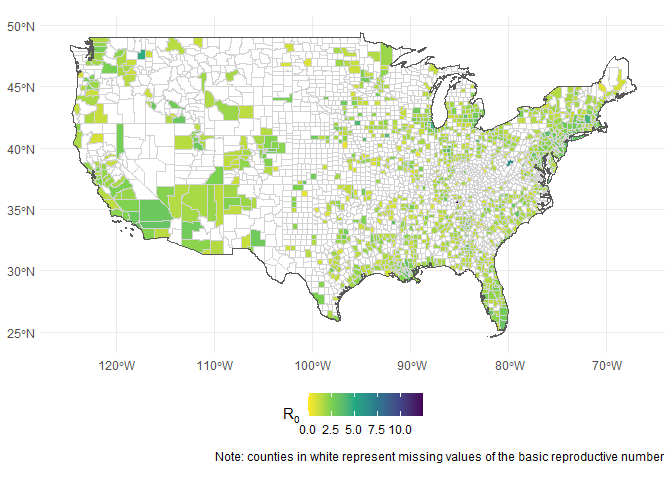
\includegraphics[width=1\linewidth]{R0-Density-Reanalysis_files/figure-latex/R0-map-1} \caption{\label{fig:R0-map}Basic reproductive rate in US counties (Alaska, Hawaii, Puerto Rico, and territories not shown).}\label{fig:R0-map}
\end{figure}

SWN used for their multivariate analysis mixed linear models. This is a
reasonable modelling choice: \(R_0\) is an interval-ratio variable that
is suitably modeled using linear regression; further, as SWN note there
is a likelihood that the process in not independent ``among counties
within each state, potentially due to variable resource allocation and
differing health systems across states'' (p.~3). A mixed linear model
accounts for this by introducing random components (in the case of SNW,
random intercepts at the state level). SWN estimated various models with
different combinations of variables, including median household income
and prevalence of travel by private transportation. These are sensible
controls, given potential variations in behavior: people in more
affluent counties may have greater opportunities to work from home, and
use of private transportation reduces contact with strangers. Moreover,
they also conducted various sensitivity analyses. After these efforts,
SNW conclude that there is a positive association between the basic
reproductive number and population density at the level of counties in
the US.

Table \ref{tab:swn-results} replicates the first three models of SWN
(the fourth model did not have any significant variables; see Table 1 in
SNW). It is possible to verify that the results match with the minor
(and irrelevant) exception of the magnitude of the coefficient for
travel by private transportation, which is due to a difference in the
input (here the variable is one percent units, whereas in SWN it was ten
percent units). The intercept in these models is a random variable, and
the standard deviation is reported in the fourth row of Table
\ref{tab:swn-results}. It is useful to map the random intercepts: as
seen in Figure \ref{fig:random-terms-map}, other things being equal,
counties in Texas tended to have somewhat lower values of \(R_0\) (i.e.,
a negative random intercept), whereas counties in South Dakota tended to
have higher values of \(R_0\). The key of the analysis, that population
density has a positive association with the basic reproductive number,
is verified. But is it really?

\begin{table}

\caption{\label{tab:tabulate-swn-results}\label{tab:swn-results}Replicating SWN: Models 1-3}
\centering
\resizebox{\linewidth}{!}{
\begin{tabular}[t]{lllllrl}
\toprule
\multicolumn{1}{c}{ } & \multicolumn{2}{c}{Model 1} & \multicolumn{2}{c}{Model 2} & \multicolumn{2}{c}{Model 3} \\
\cmidrule(l{3pt}r{3pt}){2-3} \cmidrule(l{3pt}r{3pt}){4-5} \cmidrule(l{3pt}r{3pt}){6-7}
Variable & beta & 95\% CI & beta & 95\% CI & beta & 95\% CI\\
\midrule
Intercept & 2.274 & [2.167, 2.381] & 3.347 & [2.676, 4.018] & 3.386 & [2.614, 4.157]\\
Log of population density & 0.162 & [0.133, 0.191] & 0.145 & [0.115, 0.176] & 0.147 & [0.113, 0.18]\\
Percent of private transportation &  &  & -0.013 & [-0.02, -0.005] & -0.013 & [-0.021, -0.005]\\
Median household income (\$10,000) &  &  &  &  & -0.003 & [-0.033, 0.026]\\
Standard deviation (Intercept) & 0.166 & [0.108, 0.254] & 0.136 & [0.081, 0.229] & 0.137 & [0.081, 0.232]\\
\addlinespace
Within-group standard error & 0.665 & [0.638, 0.693] & 0.665 & [0.638, 0.693] & 0.665 & [0.638, 0.694]\\
\bottomrule
\end{tabular}}
\end{table}

\begin{figure}
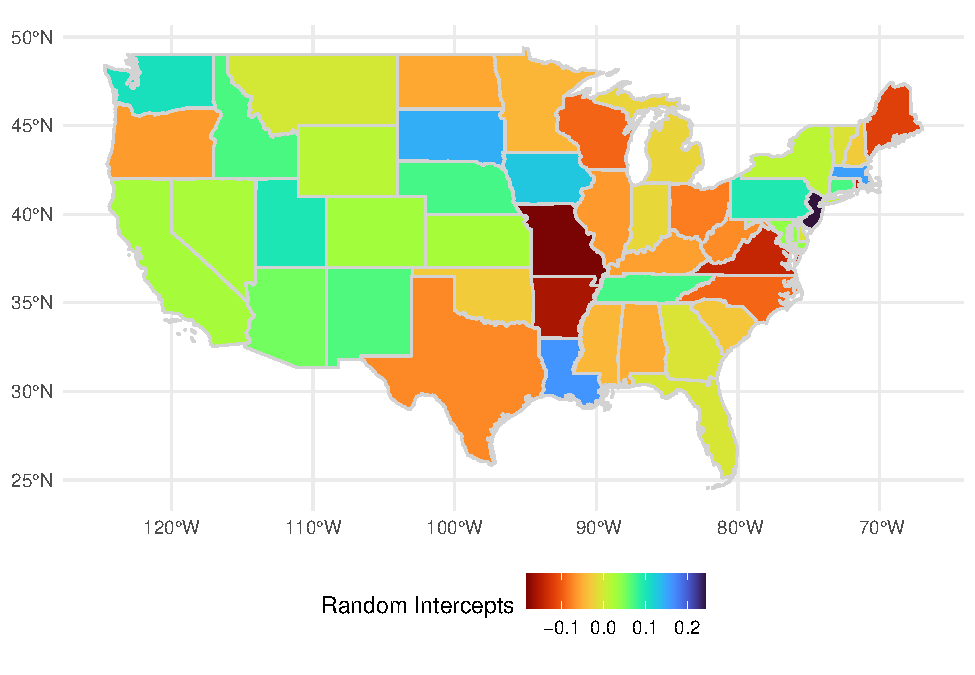
\includegraphics[width=1\linewidth]{R0-Density-Reanalysis_files/figure-latex/random-terms-map-1} \caption{\label{fig:random-terms-map}Random intercepts of Model 3 (Alaska, Hawaii, Puerto Rico, and territories not shown).}\label{fig:random-terms-map}
\end{figure}

\hypertarget{expanding-on-swn}{%
\section{Expanding on SWN}\label{expanding-on-swn}}

Thanks to the availability of code and data, it was possible to verify
the results reported by SWN. As noted earlier, though, an experienced
spatial modeller would have asked themselves about the implications of
the spatial sampling procedure used by SWN. The decision to use a sample
of counties with reliable basic reproductive numbers, although seemingly
sensible, results in a non-random sampling scheme. Turning our attention
back to Figure \ref{fig:R0-map}, we see that many counties without
reliable values of \(R_0\) are in more rural, less dense parts of the
United States. The fact that \(R_0\) could not be accurately computed in
those counties does not mean that there was no transmission of the
virus: it simply means that we do not know with precision whether that
was the case. The low number of cases may be related to low population
and/or low population density. This is intriguing, to say the least: by
excluding cases in a non-random way such as this, we are in effect
\emph{truncating} the sample.

The issue with sample truncation is that parameter estimates can become
unreliable.

Alas, despite decades' worth of developments in the field of
geographical analysis, not all research presented to date has used
proper methods for the study of COVID-19. While the answer to the
question ``do spatial effects really matter in regression analysis'' was
definitively answered in the positive at least 40 years ago, in practice
many researchers continue to ignore the pitfalls of ignoring them. In
this paper, I present a reanalysis of the data used by Sy et al.~(2021)
to study the correlations between the basic reproductive number of
COVID-19 and population density in counties. I highlight two related
issues: non-systematic sampling in space and spatial autocorrelation.
The reanalysis is based on the use of tobit models to account for
non-systematic sampling, and spatially autoregressive tobit models to
account for spatial autocorrelation in the data generation process. The
reanalysis highlights the importance of openness and reproducibility in
COVID-19 research. Finally, the results provide a sobering example of
the risks of not using appropriate methods in the analysis of
geographical data. Furthermore,

\hypertarget{fit-tobit-version-of-models}{%
\subsection{Fit tobit version of
models}\label{fit-tobit-version-of-models}}

\begin{table}

\caption{\label{tab:unnamed-chunk-3}\label{tab:tobit-results}Marginal effects of sample selection models}
\centering
\resizebox{\linewidth}{!}{
\begin{tabular}[t]{lllllrl}
\toprule
\multicolumn{1}{c}{ } & \multicolumn{2}{c}{Tobit Model 1} & \multicolumn{2}{c}{Tobit Model 2} & \multicolumn{2}{c}{Tobit Model 3} \\
\cmidrule(l{3pt}r{3pt}){2-3} \cmidrule(l{3pt}r{3pt}){4-5} \cmidrule(l{3pt}r{3pt}){6-7}
Variable & m.e. & 95\% CI & m.e. & 95\% CI & m.e. & 95\% CI\\
\midrule
Log of population density & 0.264 & [0.246, 0.281] & 0.264 & [0.247, 0.281] & 0.233 & [0.216, 0.25]\\
Percent of private transportation &  &  & 0.006 & [0.002, 0.01] & 0.014 & [0.01, 0.019]\\
Median household income (\$10,000) &  &  &  &  & 0.105 & [0.087, 0.122]\\
\bottomrule
\end{tabular}}
\end{table}

\hypertarget{spatially-autoregressive-tobit}{%
\subsection{Spatially autoregressive
tobit}\label{spatially-autoregressive-tobit}}

Fit spatially autoregressive tobit:

\hypertarget{conclusion}{%
\section{Conclusion}\label{conclusion}}

Words go here.

\hypertarget{references}{%
\section*{References}\label{references}}
\addcontentsline{toc}{section}{References}

\hypertarget{refs}{}
\begin{CSLReferences}{0}{0}
\leavevmode\hypertarget{ref-Fraser2021evolving}{}%
\CSLLeftMargin{1. }
\CSLRightInline{Fraser N, Brierley L, Dey G, Polka JK, Pálfy M, Nanni F,
et al. The evolving role of preprints in the dissemination of COVID-19
research and their impact on the science communication landscape. PLOS
Biology. 2021;19: e3000959.
doi:\href{https://doi.org/10.1371/journal.pbio.3000959}{10.1371/journal.pbio.3000959}}

\leavevmode\hypertarget{ref-Kwon2021swamped}{}%
\CSLLeftMargin{2. }
\CSLRightInline{Kwon D. How swamped preprint servers are blocking bad
coronavirus research. Nature. 2020;581: 130--132. }

\leavevmode\hypertarget{ref-Vlasschaert2020proliferation}{}%
\CSLLeftMargin{3. }
\CSLRightInline{Vlasschaert C, Topf JM, Hiremath S. Proliferation of
papers and preprints during the coronavirus disease 2019 pandemic:
Progress or problems with peer review? Advances in Chronic Kidney
Disease. 2020;27: 418--426.
doi:\href{https://doi.org/10.1053/j.ackd.2020.08.003}{10.1053/j.ackd.2020.08.003}}

\leavevmode\hypertarget{ref-Anazco2021publication}{}%
\CSLLeftMargin{4. }
\CSLRightInline{Añazco D, Nicolalde B, Espinosa I, Camacho J, Mushtaq M,
Gimenez J, et al. Publication rate and citation counts for preprints
released during the COVID-19 pandemic: The good, the bad and the ugly.
PeerJ. 2021;9: e10927.
doi:\href{https://doi.org/10.7717/peerj.10927}{10.7717/peerj.10927}}

\leavevmode\hypertarget{ref-Bramstedt2020carnage}{}%
\CSLLeftMargin{5. }
\CSLRightInline{Bramstedt KA. The carnage of substandard research during
the COVID-19 pandemic: A call for quality. Journal of Medical Ethics.
2020;46: 803--807.
doi:\href{https://doi.org/10.1136/medethics-2020-106494}{10.1136/medethics-2020-106494}}

\leavevmode\hypertarget{ref-Broggini2017reproducible}{}%
\CSLLeftMargin{6. }
\CSLRightInline{Broggini F, Dellinger J, Fomel S, Liu Y. Reproducible
research: Geophysics papers of the future - introduction. Geophysics.
2017;82.
doi:\href{https://doi.org/10.1190/geo2017-0918-spseintro.1}{10.1190/geo2017-0918-spseintro.1}}

\leavevmode\hypertarget{ref-Ince2012case}{}%
\CSLLeftMargin{7. }
\CSLRightInline{Ince DC, Hatton L, Graham-Cumming J. The case for open
computer programs. Nature. 2012;482: 485--488.
doi:\href{https://doi.org/10.1038/nature10836}{10.1038/nature10836}}

\leavevmode\hypertarget{ref-Ioannidis2014increasing}{}%
\CSLLeftMargin{8. }
\CSLRightInline{Ioannidis JPA, Greenland S, Hlatky MA, Khoury MJ,
Macleod MR, Moher D, et al. Increasing value and reducing waste in
research design, conduct, and analysis. Lancet. 2014;383: 166--175.
doi:\href{https://doi.org/10.1016/s0140-6736(13)62227-8}{10.1016/s0140-6736(13)62227-8}}

\leavevmode\hypertarget{ref-Brunsdon2020opening}{}%
\CSLLeftMargin{9. }
\CSLRightInline{Brunsdon C, Comber A. Opening practice: Supporting
reproducibility and critical spatial data science. Journal of
Geographical Systems. 2020;
doi:\href{https://doi.org/10.1007/s10109-020-00334-2}{10.1007/s10109-020-00334-2}}

\leavevmode\hypertarget{ref-Konkol2019examination}{}%
\CSLLeftMargin{10. }
\CSLRightInline{Konkol M, Kray C. In-depth examination of spatiotemporal
figures in open reproducible research. Cartography and Geographic
Information Science. 2019;46: 412--427.
doi:\href{https://doi.org/10.1080/15230406.2018.1512421}{10.1080/15230406.2018.1512421}}

\leavevmode\hypertarget{ref-Konkol2019computational}{}%
\CSLLeftMargin{11. }
\CSLRightInline{Konkol M, Kray C, Pfeiffer M. Computational
reproducibility in geoscientific papers: Insights from a series of
studies with geoscientists and a reproduction study. International
Journal of Geographical Information Science. 2019;33: 408--429.
doi:\href{https://doi.org/10.1080/13658816.2018.1508687}{10.1080/13658816.2018.1508687}}

\leavevmode\hypertarget{ref-Iqbal2016reproducible}{}%
\CSLLeftMargin{12. }
\CSLRightInline{Iqbal SA, Wallach JD, Khoury MJ, Schully SD, Ioannidis
JPA. Reproducible research practices and transparency across the
biomedical literature. Plos Biology. 2016;14.
doi:\href{https://doi.org/10.1371/journal.pbio.1002333}{10.1371/journal.pbio.1002333}}

\leavevmode\hypertarget{ref-Stodden2018empirical}{}%
\CSLLeftMargin{13. }
\CSLRightInline{Stodden V, Seiler J, Ma ZK. An empirical analysis of
journal policy effectiveness for computational reproducibility.
Proceedings of the National Academy of Sciences of the United States of
America. 2018;115: 2584--2589.
doi:\href{https://doi.org/10.1073/pnas.1708290115}{10.1073/pnas.1708290115}}

\leavevmode\hypertarget{ref-Sumner2020reproducibility}{}%
\CSLLeftMargin{14. }
\CSLRightInline{Sumner J, Haynes L, Nathan S, Hudson-Vitale C, McIntosh
LD. Reproducibility and reporting practices in COVID-19 preprint
manuscripts. medRxiv. 2020; 2020.03.24.20042796.
doi:\href{https://doi.org/10.1101/2020.03.24.20042796}{10.1101/2020.03.24.20042796}}

\leavevmode\hypertarget{ref-Gustot2020quality}{}%
\CSLLeftMargin{15. }
\CSLRightInline{Gustot T. Quality and reproducibility during the
COVID-19 pandemic. JHEP Rep. 2020;2: 100141.
doi:\href{https://doi.org/10.1016/j.jhepr.2020.100141}{10.1016/j.jhepr.2020.100141}}

\leavevmode\hypertarget{ref-Herndon2014high}{}%
\CSLLeftMargin{16. }
\CSLRightInline{Herndon T, Ash M, Pollin R. Does high public debt
consistently stifle economic growth? A critique of reinhart and rogoff.
Cambridge Journal of Economics. 2014;38: 257--279.
doi:\href{https://doi.org/10.1093/cje/bet075}{10.1093/cje/bet075}}

\leavevmode\hypertarget{ref-Basu2017ten}{}%
\CSLLeftMargin{17. }
\CSLRightInline{Basu S, Carney MA, Kenworthy NJ. Ten years after the
financial crisis: The long reach of austerity and its global impacts on
health. Social Science \& Medicine. 2017;187: 203--207.
doi:\href{https://doi.org/10.1016/j.socscimed.2017.06.026}{10.1016/j.socscimed.2017.06.026}}

\leavevmode\hypertarget{ref-Florida2020how}{}%
\CSLLeftMargin{18. }
\CSLRightInline{Florida R, Glaeser E, Sharif M, Bedi K, Campanella T,
Chee C, et al. How life in our cities will look after the coronavirus
pandemic. Foreign Policy. 2020;1. Available:
\url{https://foreignpolicy.com/2020/05/01/future-of-cities-urban-life-after-coronavirus-pandemic/}}

\leavevmode\hypertarget{ref-Sy2021population}{}%
\CSLLeftMargin{19. }
\CSLRightInline{Sy KTL, White LF, Nichols BE. Population density and
basic reproductive number of COVID-19 across united states counties.
PLOS ONE. 2021;16: e0249271.
doi:\href{https://doi.org/10.1371/journal.pone.0249271}{10.1371/journal.pone.0249271}}

\leavevmode\hypertarget{ref-Moore1970urban}{}%
\CSLLeftMargin{20. }
\CSLRightInline{Moore EG, Brown LA. Urban acquaintance fields: An
evaluation of a spatial model. Environment and Planning. 1970;2:
443--454. Available:
\url{http://www.envplan.com/abstract.cgi?id=a020443}}

\leavevmode\hypertarget{ref-Moore1970some}{}%
\CSLLeftMargin{21. }
\CSLRightInline{Moore EG. Some spatial properties of urban contact
fields. Geographical Analysis. 1970;2: 376--386. }

\leavevmode\hypertarget{ref-Farber2011running}{}%
\CSLLeftMargin{22. }
\CSLRightInline{Farber S, Páez A. Running to stay in place: The time-use
implications of automobile oriented land-use and travel. Journal of
Transport Geography. 2011;19: 782--793.
doi:\href{https://doi.org/10.1016/j.jtrangeo.2010.09.008}{10.1016/j.jtrangeo.2010.09.008}}

\leavevmode\hypertarget{ref-Rocklov2020high}{}%
\CSLLeftMargin{23. }
\CSLRightInline{Rocklöv J, Sjödin H. High population densities catalyse
the spread of COVID-19. Journal of Travel Medicine. 2020;27.
doi:\href{https://doi.org/10.1093/jtm/taaa038}{10.1093/jtm/taaa038}}

\leavevmode\hypertarget{ref-Li2018effect}{}%
\CSLLeftMargin{24. }
\CSLRightInline{Li R, Richmond P, Roehner BM. Effect of population
density on epidemics. Physica A: Statistical Mechanics and its
Applications. 2018;510: 713--724.
doi:\href{https://doi.org/10.1016/j.physa.2018.07.025}{10.1016/j.physa.2018.07.025}}

\leavevmode\hypertarget{ref-Cruz2020exploring}{}%
\CSLLeftMargin{25. }
\CSLRightInline{Cruz CJP, Ganly R, Li Z, Gietel-Basten S. Exploring the
young demographic profile of COVID-19 cases in hong kong: Evidence from
migration and travel history data. PLOS ONE. 2020;15: e0235306.
doi:\href{https://doi.org/10.1371/journal.pone.0235306}{10.1371/journal.pone.0235306}}

\leavevmode\hypertarget{ref-Micallef2020first}{}%
\CSLLeftMargin{26. }
\CSLRightInline{Micallef S, Piscopo TV, Casha R, Borg D, Vella C, Zammit
M-A, et al. The first wave of COVID-19 in malta; a national
cross-sectional study. PLOS ONE. 2020;15: e0239389.
doi:\href{https://doi.org/10.1371/journal.pone.0239389}{10.1371/journal.pone.0239389}}

\leavevmode\hypertarget{ref-Gomez2021infekta}{}%
\CSLLeftMargin{27. }
\CSLRightInline{Gomez J, Prieto J, Leon E, Rodríguez A. INFEKTA---an
agent-based model for transmission of infectious diseases: The COVID-19
case in bogotá, colombia. PLOS ONE. 2021;16: e0245787.
doi:\href{https://doi.org/10.1371/journal.pone.0245787}{10.1371/journal.pone.0245787}}

\leavevmode\hypertarget{ref-Noland1995perceived}{}%
\CSLLeftMargin{28. }
\CSLRightInline{Noland RB. PERCEIVED RISK AND MODAL CHOICE - RISK
COMPENSATION IN TRANSPORTATION SYSTEM. Accident Analysis and Prevention.
1995;27: 503--521.
doi:\href{https://doi.org/10.1016/0001-4575(94)00087-3}{10.1016/0001-4575(94)00087-3}}

\leavevmode\hypertarget{ref-Richens2000condoms}{}%
\CSLLeftMargin{29. }
\CSLRightInline{Richens J, Imrie J, Copas A. Condoms and seat belts: The
parallels and the lessons. Lancet. 2000;355: 400--403.
doi:\href{https://doi.org/10.1016/s0140-6736(99)09109-6}{10.1016/s0140-6736(99)09109-6}}

\leavevmode\hypertarget{ref-Phillips2011risk}{}%
\CSLLeftMargin{30. }
\CSLRightInline{Phillips RO, Fyhri A, Sagberg F. Risk compensation and
bicycle helmets. Risk Analysis. 2011;31: 1187--1195.
doi:\href{https://doi.org/10.1111/j.1539-6924.2011.01589.x}{10.1111/j.1539-6924.2011.01589.x}}

\leavevmode\hypertarget{ref-Chauhan2021covid}{}%
\CSLLeftMargin{31. }
\CSLRightInline{Chauhan RS, Capasso da Silva D, Salon D, Shamshiripour
A, Rahimi E, Sutradhar U, et al. COVID-19 related attitudes and risk
perceptions across urban, rural, and suburban areas in the united
states. Findings. Network Design Lab; 2021;
doi:\href{https://doi.org/10.32866/001c.23714}{10.32866/001c.23714}}

\leavevmode\hypertarget{ref-Paez2020spatio}{}%
\CSLLeftMargin{32. }
\CSLRightInline{Paez A, Lopez FA, Menezes T, Cavalcanti R, Pitta MG da
R. A spatio-temporal analysis of the environmental correlates of
COVID-19 incidence in spain. Geographical Analysis. 2020;n/a.
doi:\href{https://doi.org/10.1111/gean.12241}{10.1111/gean.12241}}

\leavevmode\hypertarget{ref-Hamidi2020density}{}%
\CSLLeftMargin{33. }
\CSLRightInline{Hamidi S, Sabouri S, Ewing R. Does density aggravate the
COVID-19 pandemic? Journal of the American Planning Association.
2020;86: 495--509.
doi:\href{https://doi.org/10.1080/01944363.2020.1777891}{10.1080/01944363.2020.1777891}}

\leavevmode\hypertarget{ref-Jamal2020Changes}{}%
\CSLLeftMargin{34. }
\CSLRightInline{Jamal S, Paez A. Changes in trip-making frequency by
mode during COVID-19. Findings. Network Design Lab; 2020;
doi:\href{https://doi.org/10.32866/001c.17977}{10.32866/001c.17977}}

\leavevmode\hypertarget{ref-Harris2021Changes}{}%
\CSLLeftMargin{35. }
\CSLRightInline{Harris MA, Branion-Calles M. Changes in commute mode
attributed to COVID-19 risk in canadian national survey data. Findings.
Network Design Lab; 2021;
doi:\href{https://doi.org/10.32866/001c.19088}{10.32866/001c.19088}}

\leavevmode\hypertarget{ref-Molloy2020Tracing}{}%
\CSLLeftMargin{36. }
\CSLRightInline{Molloy J, Tchervenkov C, Hintermann B, Axhausen KW.
Tracing the sars-CoV-2 impact: The first month in switzerland. Findings.
Network Design Lab; 2020;
doi:\href{https://doi.org/10.32866/001c.12903}{10.32866/001c.12903}}

\leavevmode\hypertarget{ref-Feyman2020effectiveness}{}%
\CSLLeftMargin{37. }
\CSLRightInline{Feyman Y, Bor J, Raifman J, Griffith KN. Effectiveness
of COVID-19 shelter-in-place orders varied by state. PLOS ONE. 2020;15:
e0245008.
doi:\href{https://doi.org/10.1371/journal.pone.0245008}{10.1371/journal.pone.0245008}}

\leavevmode\hypertarget{ref-Praharaj2020Using}{}%
\CSLLeftMargin{38. }
\CSLRightInline{Praharaj S, King D, Pettit C, Wentz E. Using aggregated
mobility data to measure the effect of COVID-19 policies on mobility
changes in sydney, london, phoenix, and pune. Findings. Network Design
Lab; 2020;
doi:\href{https://doi.org/10.32866/001c.17590}{10.32866/001c.17590}}

\leavevmode\hypertarget{ref-Paez2020using}{}%
\CSLLeftMargin{39. }
\CSLRightInline{Paez A. Using google community mobility reports to
investigate the incidence of COVID-19 in the united states. Findings.
2020; doi:\url{https://doi.org/10.32866/001c.12976}}

\leavevmode\hypertarget{ref-Noland2021mobility}{}%
\CSLLeftMargin{40. }
\CSLRightInline{Noland RB. Mobility and the effective reproduction rate
of COVID-19. Journal of Transport \& Health. 2021;20: 101016.
doi:\url{https://doi.org/10.1016/j.jth.2021.101016}}

\leavevmode\hypertarget{ref-Bhadra2021impact}{}%
\CSLLeftMargin{41. }
\CSLRightInline{Bhadra A, Mukherjee A, Sarkar K. Impact of population
density on covid-19 infected and mortality rate in india. Modeling Earth
Systems and Environment. 2021;7: 623--629.
doi:\href{https://doi.org/10.1007/s40808-020-00984-7}{10.1007/s40808-020-00984-7}}

\leavevmode\hypertarget{ref-Kadi2020population}{}%
\CSLLeftMargin{42. }
\CSLRightInline{Kadi N, Khelfaoui M. Population density, a factor in the
spread of COVID-19 in algeria: Statistic study. Bulletin of the National
Research Centre. 2020;44.
doi:\href{https://doi.org/10.1186/s42269-020-00393-x}{10.1186/s42269-020-00393-x}}

\leavevmode\hypertarget{ref-Pequeno2020air}{}%
\CSLLeftMargin{43. }
\CSLRightInline{Pequeno P, Mendel B, Rosa C, Bosholn M, Souza JL,
Baccaro F, et al. Air transportation, population density and temperature
predict the spread of COVID-19 in brazil. PeerJ. 2020;8: e9322.
doi:\href{https://doi.org/10.7717/peerj.9322}{10.7717/peerj.9322}}

\leavevmode\hypertarget{ref-Fielding2020social}{}%
\CSLLeftMargin{44. }
\CSLRightInline{Fielding-Miller RK, Sundaram ME, Brouwer K. Social
determinants of COVID-19 mortality at the county level. PLOS ONE.
2020;15: e0240151.
doi:\href{https://doi.org/10.1371/journal.pone.0240151}{10.1371/journal.pone.0240151}}

\leavevmode\hypertarget{ref-Roy2020factors}{}%
\CSLLeftMargin{45. }
\CSLRightInline{Roy S, Ghosh P. Factors affecting COVID-19 infected and
death rates inform lockdown-related policymaking. PLOS ONE. 2020;15:
e0241165.
doi:\href{https://doi.org/10.1371/journal.pone.0241165}{10.1371/journal.pone.0241165}}

\leavevmode\hypertarget{ref-Wong2020spreading}{}%
\CSLLeftMargin{46. }
\CSLRightInline{Wong DWS, Li Y. Spreading of COVID-19: Density matters.
PLOS ONE. 2020;15: e0242398.
doi:\href{https://doi.org/10.1371/journal.pone.0242398}{10.1371/journal.pone.0242398}}

\leavevmode\hypertarget{ref-Sun2020impacts}{}%
\CSLLeftMargin{47. }
\CSLRightInline{Sun Z, Zhang H, Yang Y, Wan H, Wang Y. Impacts of
geographic factors and population density on the COVID-19 spreading
under the lockdown policies of china. Science of The Total Environment.
2020;746: 141347.
doi:\href{https://doi.org/10.1016/j.scitotenv.2020.141347}{10.1016/j.scitotenv.2020.141347}}

\leavevmode\hypertarget{ref-Skorka2020macroecology}{}%
\CSLLeftMargin{48. }
\CSLRightInline{Skórka P, Grzywacz B, Moroń D, Lenda M. The macroecology
of the COVID-19 pandemic in the anthropocene. PLOS ONE. 2020;15:
e0236856.
doi:\href{https://doi.org/10.1371/journal.pone.0236856}{10.1371/journal.pone.0236856}}

\leavevmode\hypertarget{ref-White2020state}{}%
\CSLLeftMargin{49. }
\CSLRightInline{White ER, Hébert-Dufresne L. State-level variation of
initial COVID-19 dynamics in the united states. PLOS ONE. 2020;15:
e0240648.
doi:\href{https://doi.org/10.1371/journal.pone.0240648}{10.1371/journal.pone.0240648}}

\leavevmode\hypertarget{ref-Khavarian2021high}{}%
\CSLLeftMargin{50. }
\CSLRightInline{Khavarian-Garmsir AR, Sharifi A, Moradpour N. Are
high-density districts more vulnerable to the COVID-19 pandemic?
Sustainable Cities and Society. 2021;70: 102911.
doi:\href{https://doi.org/10.1016/j.scs.2021.102911}{10.1016/j.scs.2021.102911}}

\leavevmode\hypertarget{ref-Hamidi2020longitudinal}{}%
\CSLLeftMargin{51. }
\CSLRightInline{Hamidi S, Ewing R, Sabouri S. Longitudinal analyses of
the relationship between development density and the COVID-19 morbidity
and mortality rates: Early evidence from 1,165 metropolitan counties in
the united states. Health \& Place. 2020;64: 102378.
doi:\href{https://doi.org/10.1016/j.healthplace.2020.102378}{10.1016/j.healthplace.2020.102378}}

\leavevmode\hypertarget{ref-Lee2020human}{}%
\CSLLeftMargin{52. }
\CSLRightInline{Lee M, Zhao J, Sun Q, Pan Y, Zhou W, Xiong C, et al.
Human mobility trends during the early stage of the COVID-19 pandemic in
the united states. PLOS ONE. 2020;15: e0241468.
doi:\href{https://doi.org/10.1371/journal.pone.0241468}{10.1371/journal.pone.0241468}}

\leavevmode\hypertarget{ref-Amadu2021assessing}{}%
\CSLLeftMargin{53. }
\CSLRightInline{Amadu I, Ahinkorah BO, Afitiri A-R, Seidu A-A, Ameyaw
EK, Hagan JE, et al. Assessing sub-regional-specific strengths of
healthcare systems associated with COVID-19 prevalence, deaths and
recoveries in africa. PLOS ONE. 2021;16: e0247274.
doi:\href{https://doi.org/10.1371/journal.pone.0247274}{10.1371/journal.pone.0247274}}

\leavevmode\hypertarget{ref-Feng2020spread}{}%
\CSLLeftMargin{54. }
\CSLRightInline{Feng Y, Li Q, Tong X, Wang R, Zhai S, Gao C, et al.
Spatiotemporal spread pattern of the COVID-19 cases in china. PLOS ONE.
2020;15: e0244351.
doi:\href{https://doi.org/10.1371/journal.pone.0244351}{10.1371/journal.pone.0244351}}

\leavevmode\hypertarget{ref-Inbaraj2021seroprevalence}{}%
\CSLLeftMargin{55. }
\CSLRightInline{Inbaraj LR, George CE, Chandrasingh S. Seroprevalence of
COVID-19 infection in a rural district of south india: A
population-based seroepidemiological study. PLOS ONE. 2021;16: e0249247.
doi:\href{https://doi.org/10.1371/journal.pone.0249247}{10.1371/journal.pone.0249247}}

\leavevmode\hypertarget{ref-Souris2020covid}{}%
\CSLLeftMargin{56. }
\CSLRightInline{Souris M, Gonzalez J-P. COVID-19: Spatial analysis of
hospital case-fatality rate in france. PLOS ONE. 2020;15: e0243606.
doi:\href{https://doi.org/10.1371/journal.pone.0243606}{10.1371/journal.pone.0243606}}

\leavevmode\hypertarget{ref-Ahmad2020association}{}%
\CSLLeftMargin{57. }
\CSLRightInline{Ahmad K, Erqou S, Shah N, Nazir U, Morrison AR,
Choudhary G, et al. Association of poor housing conditions with COVID-19
incidence and mortality across US counties. PLOS ONE. 2020;15: e0241327.
doi:\href{https://doi.org/10.1371/journal.pone.0241327}{10.1371/journal.pone.0241327}}

\leavevmode\hypertarget{ref-Noury2021how}{}%
\CSLLeftMargin{58. }
\CSLRightInline{Noury A, François A, Gergaud O, Garel A. How does
COVID-19 affect electoral participation? Evidence from the french
municipal elections. PLOS ONE. 2021;16: e0247026.
doi:\href{https://doi.org/10.1371/journal.pone.0247026}{10.1371/journal.pone.0247026}}

\leavevmode\hypertarget{ref-Wang2021transmission}{}%
\CSLLeftMargin{59. }
\CSLRightInline{Wang F, Tan Z, Yu Z, Yao S, Guo C. Transmission and
control pressure analysis of the COVID-19 epidemic situation using
multisource spatio-temporal big data. PLOS ONE. 2021;16: e0249145.
doi:\href{https://doi.org/10.1371/journal.pone.0249145}{10.1371/journal.pone.0249145}}

\leavevmode\hypertarget{ref-Brandtner2021creatures}{}%
\CSLLeftMargin{60. }
\CSLRightInline{Brandtner C, Bettencourt LMA, Berman MG, Stier AJ.
Creatures of the state? Metropolitan counties compensated for state
inaction in initial u.s. Response to COVID-19 pandemic. PLOS ONE.
2021;16: e0246249.
doi:\href{https://doi.org/10.1371/journal.pone.0246249}{10.1371/journal.pone.0246249}}

\leavevmode\hypertarget{ref-Stephens2021impact}{}%
\CSLLeftMargin{61. }
\CSLRightInline{Stephens KE, Chernyavskiy P, Bruns DR. Impact of
altitude on COVID-19 infection and death in the united states: A
modeling and observational study. PLOS ONE. 2021;16: e0245055.
doi:\href{https://doi.org/10.1371/journal.pone.0245055}{10.1371/journal.pone.0245055}}

\end{CSLReferences}

\nolinenumbers


\end{document}
